\documentclass{beamer}
% Sans animations
%\documentclass[handout]{beamer}

\usepackage{tikz}
\usepackage{pgfplots}
\tikzstyle{every picture}+=[remember picture]

\setbeamertemplate{footline}[frame number]

\title{DEV1 : les modules en Go}
\author{}
\date{loig.jezequel@univ-nantes.fr}

\begin{document}

\frame{
\maketitle
}

\frame{
\frametitle{Objectifs du cours}
\begin{block}{Pour l'instant}
\begin{itemize}
  \item Un fichier par exercice~: pas pratique pour un gros projet.
  \item Toujours un main~: pas adapté pour une bibliothèque.
\end{itemize}
\end{block}

\begin{alertblock}{Bibliothèque}
Ensemble de fonctions prêtes à être utilisées par des programmes.
\end{alertblock}

\begin{block}{Le cours d'aujourd'hui}
  \begin{itemize}
    \item Comment organiser son code pour un gros projet ?
    \item Comment fabriquer ses propres bibliothèques ?
    \item Comment gérer les dépendances de son code à des bibliothèques externes ?
  \end{itemize}
\end{block}
}

\frame{
\frametitle{La solution à tous nos problèmes~: les modules}

\begin{block}{Organiser son code}
Au sein d'un module on peut organiser son code en plusieurs fichiers et dossiers pour bien \alert{séparer les différentes fonctionnalités}.
\end{block}

\begin{block}{Fabriquer ses bibliothèques}
Un module est un moyen de \alert{compartimenter} son code et de le \alert{distribuer} aux autres programmeurs.
\end{block}

\begin{block}{Gérer les dépendances}
Un module \alert{enregistre les bibliothèques utilisées} par le code qu'il contient avec des informations précises sur la \alert{version} exacte à utiliser
\end{block}

}

\frame{
\frametitle{Qu'est-ce qu'un module ?}

\begin{block}{Paquet (\emph{package})}
Collection de fichiers sources, tous situés dans le même répertoire, et qui sont compilés ensemble.
\begin{itemize}
\item Code partagé entre les fichiers (une fonction définie dans un fichier est utilisable dans un autre).
\item Unité d'importation (en Go on importe des paquets).
\end{itemize}
\end{block}

\begin{block}{Module}
Collection de paquets qui sont publiés, versionnés et distribués ensemble.
\begin{itemize}
\item Identifié par un chemin (\emph{module path}).
\item Fichier go.mod à la racine.
\item Fichier go.sum à la racine.
\end{itemize}
\end{block}
}

\frame{
\frametitle{Organisation d'un module}

\begin{figure}
  \centering
  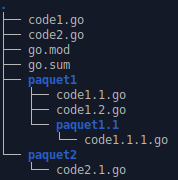
\includegraphics{arbo.png}
  \caption{Organisation classique d'un module}
\end{figure}

}

\frame{
\frametitle{Organisation d'un module, suite}

\begin{figure}
  \centering
  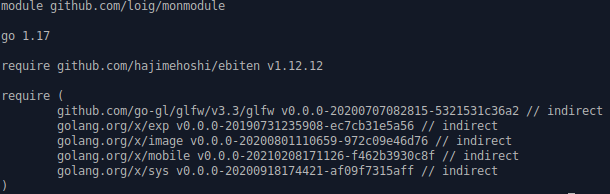
\includegraphics[width=10cm]{gomod.png}
  \caption{Contenu d'un fichier go.mod}
\end{figure}

\begin{figure}
\centering
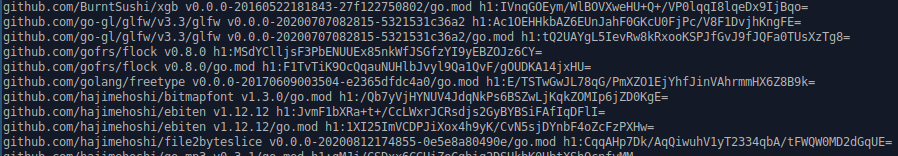
\includegraphics[width=11cm]{gosum.png}
\caption{Contenu (partiel) d'un fichier go.sum}
\end{figure}

}

\frame{
\frametitle{Créer un module}

\begin{block}{Commande (dans le dossier où sera le code)}
go mod init chemin
\end{block}

\begin{block}{Choix du chemin}
  Le chemin d'un module permettra de l'importer dans d'autres programmes.
  Il doit respecter certaines règles.
\begin{description}
  \item[Bibliothèque publique] le chemin est l'\alert{adresse où la trouver}.
  \item[Bibliothèque privée] le chemin est ce qu'on veut.
  \item[Programme exécutable] le chemin est ce qu'on veut.
\end{description}
  Ceci permet d'assurer qu'il n'y a pas deux bibliothèques (modules) utilisables par tous qui ont le même chemin.
\end{block}

}

\frame{
\frametitle{Compiler un module}

\begin{block}{Commande (à la racine du module)}
go build
\end{block}

\begin{block}{Main}
Si votre module contient de quoi s'exécuter à la racine (package main + fonction main), un exécutable du nom du module sera produit.
\end{block}

\begin{block}{Commandes alternatives (à la racine du module)}
\begin{description}
\item[Installation] go install\\
Les fichiers compilés sont placés dans l'espace de travail Go (variable d'environnement).
\item[Exécution] go run\\
Seulement si le module contient un main, il s'exécute directement.
\end{description}
\end{block}
}

\frame{
\frametitle{Créer des nouveaux paquets}

\begin{block}{Pour quoi faire ?}
Rendre le code plus lisible, mieux organisé, en le séparant en plusieurs parties plus ou moins indépendantes.
\end{block}

\begin{exampleblock}{Un exemple}
Le paquet \emph{image} de la bibliothèque standard (création et manipulation d'images en Go) contient un paquet dédié au traitement des images png et un autre dédié aux images jpeg.
\end{exampleblock}

\begin{block}{Comment ?}
\begin{enumerate}
\item Créer un dossier avec le nom du paquet,
\item faire commencer les fichiers source Go placés dans ce paquet par \emph{package xxx} où xxx est le nom du paquet.
\end{enumerate}
\end{block}

}

\frame{
\frametitle{Utiliser des paquets}

\begin{block}{Nom long pour l'importation}
Pour importer un paquet on utilise son nom long, c'est à dire le \alert{chemin du module} suivi du \alert{chemin du paquet} depuis la racine du module.
\end{block}

\begin{block}{Nom court pour l'utilisation}
Pour utiliser un paquet on se sert de son nom court, c'est à dire le nom du dossier où sont les sources (qui est aussi celui qu'on indique au début des fichiers du paquet).
\end{block}

\begin{alertblock}{Visibilité, attention}
Les fonctions/variables/types définis dans un paquet sont visibles (c'est-à-dire utilisable à l'extérieur du paquet) si et seulement si leur nom commence par une majuscule.
\end{alertblock}

}

\frame{
\frametitle{Paquets provenant d'un autre module}

\begin{block}{Bibliothèque standard}
  \begin{itemize}
    \item Nom court pour importer et utiliser.
  \end{itemize}
\end{block}

\begin{block}{Module disponible publiquement}
  \begin{itemize}
    \item Nom long pour importer (et nom court pour utiliser).
    \item Commande \alert{go mod tidy} pour récupérer automatiquement le paquet si nécessaire, ainsi que mettre à jour automatiquement go.mod et go.num.
  \end{itemize}
\end{block}

\begin{block}{Module M non disponible publiquement}
  \begin{itemize}
    \item Nom long pour importer (et nom court pour utiliser).
    \item Ajouter \alert{replace M $=>$ chemin} dans go.mod.
    \item Commande \alert{go mod tidy} pour récupérer le paquet si nécessaire, ainsi que mettre à jour automatiquement go.mod et go.num.
  \end{itemize}
\end{block}

}

\frame{
\frametitle{Quelques références}

\begin{block}{Structurer son code Go}
\url{https://golang.org/doc/code}
\end{block}

\begin{block}{Gérer les dépendances de ses programmes}
\url{https://golang.org/doc/modules/managing-dependencies}
\end{block}

\begin{block}{Fonctionnement précis des modules}
\url{https://golang.org/ref/mod}
\end{block}
}

\end{document}
